\documentclass[a4paper,12pt]{article}
\usepackage{xcolor}
\usepackage{amsmath,amsfonts,amssymb}
\usepackage{geometry}
\usepackage{fancyhdr}
\usepackage{graphicx}
\usepackage{titlesec}
\usepackage{tikz}
\usepackage{booktabs}
\usepackage{array}
\usetikzlibrary{shadows}
\usepackage{tcolorbox}
\usepackage{float}
\usepackage{lipsum}
\usepackage{mdframed}
\usepackage{pagecolor}
\usepackage{mathpazo}   % Palatino font (serif)
\usepackage{microtype}  % Better typography

\setlength{\parindent}{0pt}

% Page background color
\pagecolor{gray!10!white}

% Geometry settings
\geometry{margin=0.5in}
\pagestyle{fancy}
\fancyhf{}

% Fancy header and footer
\fancyhead[C]{\textbf{\color{blue!80}CS765 Project Part-2}}
% \fancyhead[R]{\color{blue!80}Saksham Rathi}
\fancyfoot[C]{\thepage}

% Custom Section Color and Format with Sans-serif font
\titleformat{\section}
{\sffamily\color{purple!90!black}\normalfont\Large\bfseries}
{\thesection}{1em}{}

% Custom subsection format
\titleformat{\subsection}
{\sffamily\color{cyan!80!black}\normalfont\large\bfseries}
{\thesubsection}{1em}{}

% Stylish Title with TikZ (Enhanced with gradient)
\newcommand{\cooltitle}[1]{%
\begin{tikzpicture}
\node[fill=blue!20,rounded corners=10pt,inner sep=12pt, drop shadow, top color=blue!50, bottom color=blue!30] (box)
{\Huge \bfseries \color{black} #1};
\end{tikzpicture}
}
\usepackage{float} % Add this package

\newenvironment{solution}[2][]{%
\begin{mdframed}[linecolor=blue!70!black, linewidth=2pt, roundcorner=10pt, backgroundcolor=yellow!10!white, skipabove=12pt, skipbelow=12pt]%
	\textbf{\large #2}
	\par\noindent\rule{\textwidth}{0.4pt}
}{
\end{mdframed}
}

% Document title
\title{\cooltitle{CS765 Project Part-2} \\
\LARGE \textbf{Analyzing Selfish Mining + Eclipse Attack in Blockchain P2P network} \\
{\bf Report}}
\author{{\bf Saksham Rathi (22B1003), Kavya Gupta (22B1053), Mayank Kumar (22B0933)} \\
\small Department of Computer Science, \\
Indian Institute of Technology Bombay \\}
\date{}

\begin{document}
\maketitle

\begin{solution}{Simulation Results}
	We are majorly calculating two ratios:

	\[ratio_1 = \frac{\text{Number of blocks generated by ringmaster in the longest chain at the ringmaster}}{\text{Total number of blocks in the longest chain at the ringmaster}}\]

	\[ratio_2 = \frac{\text{Number of blocks generated by ringmaster in the longest chain at the ringmaster}}{\text{Total blocks generated by the ringmaster}}\]


	(Blocks being generted by malicious nodes is essentially the same as blocks being generated by ringmaster because of our attack's design.)

	Here is the list of choices of the parameters (default):

	\begin{itemize}
		\item Number of peers (nodes) = 100
		\item Transaction Arrival Time = 10
		\item Block Arrival Time = 100
		\item Total Simulation Time = 17500
	\end{itemize}

	Now, keeping these fixed, we vary the percentage of malicious nodes, and the timeout of get requests, and collect those two ratios.

	It is worth noting that we perform all of this calculation at the ringmaster node. 
	
\end{solution}
\clearpage
\begin{solution}{Selfish Mining + Eclipse Attack}
	We varied the percentage of malicious nodes beginning from 5\% to 100\%, in steps of size 5\%. For each malicious percentage value, we tested for 6 timeout values, ranging from 10 to 400. We chose this range for timeout values, because the block inter arrival time is set to 100, so we wanted to start from a fraction of this (where many blocks will not get received) till a good multiple of this, where most blocks should get received. Also, each experiment was run for 3 iterations, and the ratio values were averaged out to prevent outliers.


	The following heatmap shows the ratios for all of these simulations:

	\begin{figure}[H]
		\centering
		\fbox{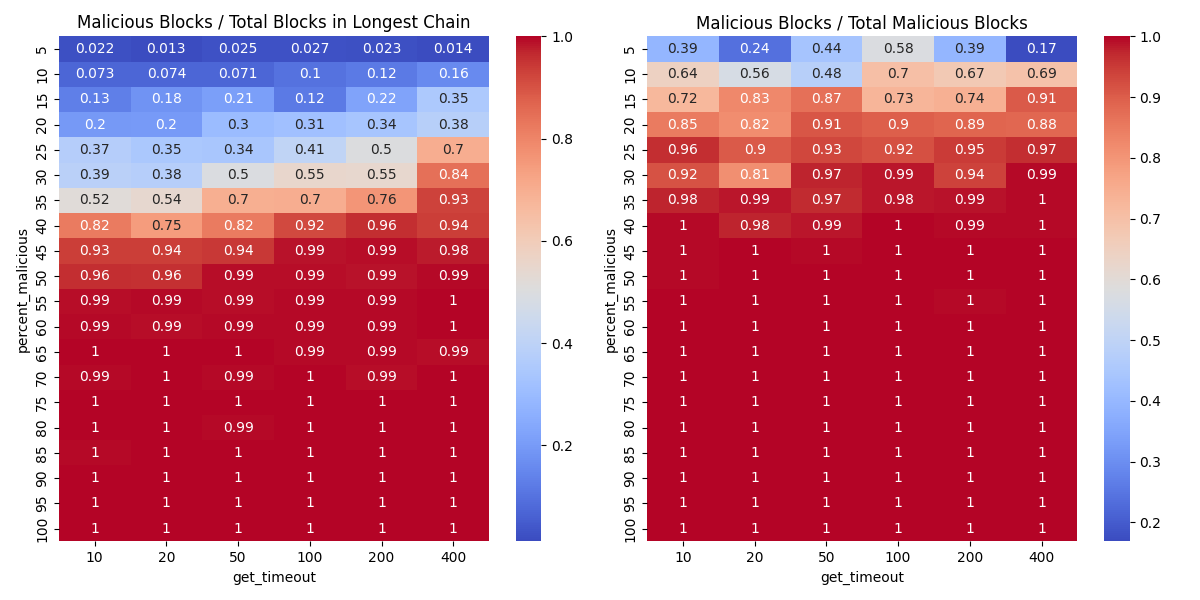
\includegraphics[width=1\textwidth, clip, trim=10 10 10 10]{images/heatmaps.png}} 
	\end{figure}

	The following inferences can be drawn from the ratio values:

	\begin{enumerate}
		\item As the number of malicious nodes increase, there is a sharp increase in the dominancy of the malicious blocks in the longest chain. 
		\item After 50\%, both the ratios reach the value 1. This essentially depicts, the 51\% attack performed, where none of the honest blocks are accepted, and only the malicious nodes are able to get the mining fees.
		\item Roughly, there is a trend of increasing ratios as the timeout increases. Multiple reasons can be attributed to this. Firstly, honest nodes need to wait for a longer time for a block to arrive. Also, a block can come later too, so more chances that the honest block is forked.
		\item For low percentages of malicious nodes, the left heatmap shows that malicious blocks constitute a small fraction of the longest chain, implying that the network remains secure against low levels of adversaries. 
		\item The right heatmap shows that even at lower levels of malicious nodes, the proportion of malicious blocks among total malicious blocks is relatively high, indicating that when malicious blocks are created, they tend to be accepted. 
		\item Higher values of \texttt{get\_timeout} generally lead to an increase in the acceptance of malicious blocks, implying that delayed responses may help malicious nodes propagate their blocks more effectively. 
	\end{enumerate}
\end{solution}
\clearpage
\begin{solution}{Selfish Mining Attack}
	For this set of experiments, we are not performing eclipse attack, that is, malicious nodes immediately forward the honest full block to the requesting node as soon as they receive a ``get'' request, for the corresponding hash. Here is the heatmap:
	\begin{figure}[H]
		\centering
		\fbox{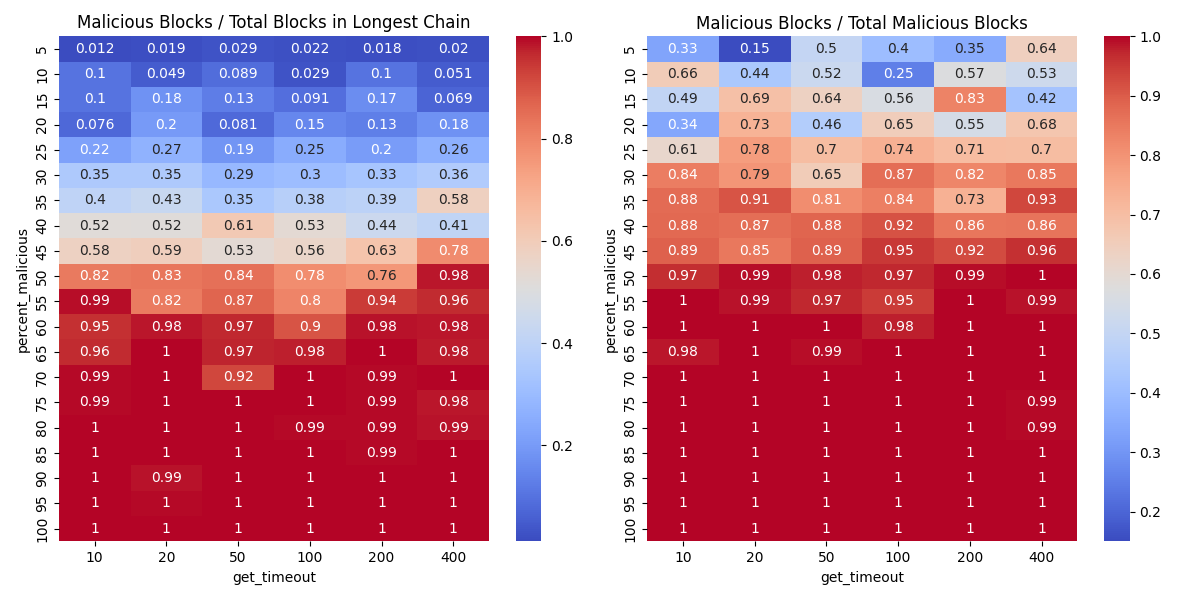
\includegraphics[width=1\textwidth, clip, trim=10 10 10 10]{images/heatmaps_eclipse.png}} 
	\end{figure}

	The following inferences can be drawn from the ratio values:

	\begin{enumerate}
		\item There appears to be a significant threshold around 45-50\% malicious mining power. Below this threshold, relatively few malicious blocks make it into the longest chain (blue regions). Above this threshold, malicious blocks dominate the chain (red regions).
		\item The right heatmap shows that at low malicious percentages (5-30\%), many produced malicious blocks are wasted (blue regions). As malicious power increases, almost all malicious blocks successfully enter the chain (red regions).
		\item Selfish Mining becomes highly effective once attackers control close to 50\% of mining power, with a sharp transition rather than a gradual one.
		\item Also, the ratio values are higher when eclipse attack is also present. This is intuitive too, because with eclipse attack, honest nodes do not get all the blocks within the timeout period, and even if they perform the mining, their chains will get forked out, by the longer private chains (or the blocks which weren't received). So, selfish mining when combined with eclipse attack is quite powerful.
	\end{enumerate}

\end{solution}
\clearpage

\begin{solution}{Network Images}
	Here is the network generated (when we pass the flag) for 100 nodes. We are ensuring the degree constraints. Orange nodes are malicious.
	\begin{figure}[H]
		\centering
		\fbox{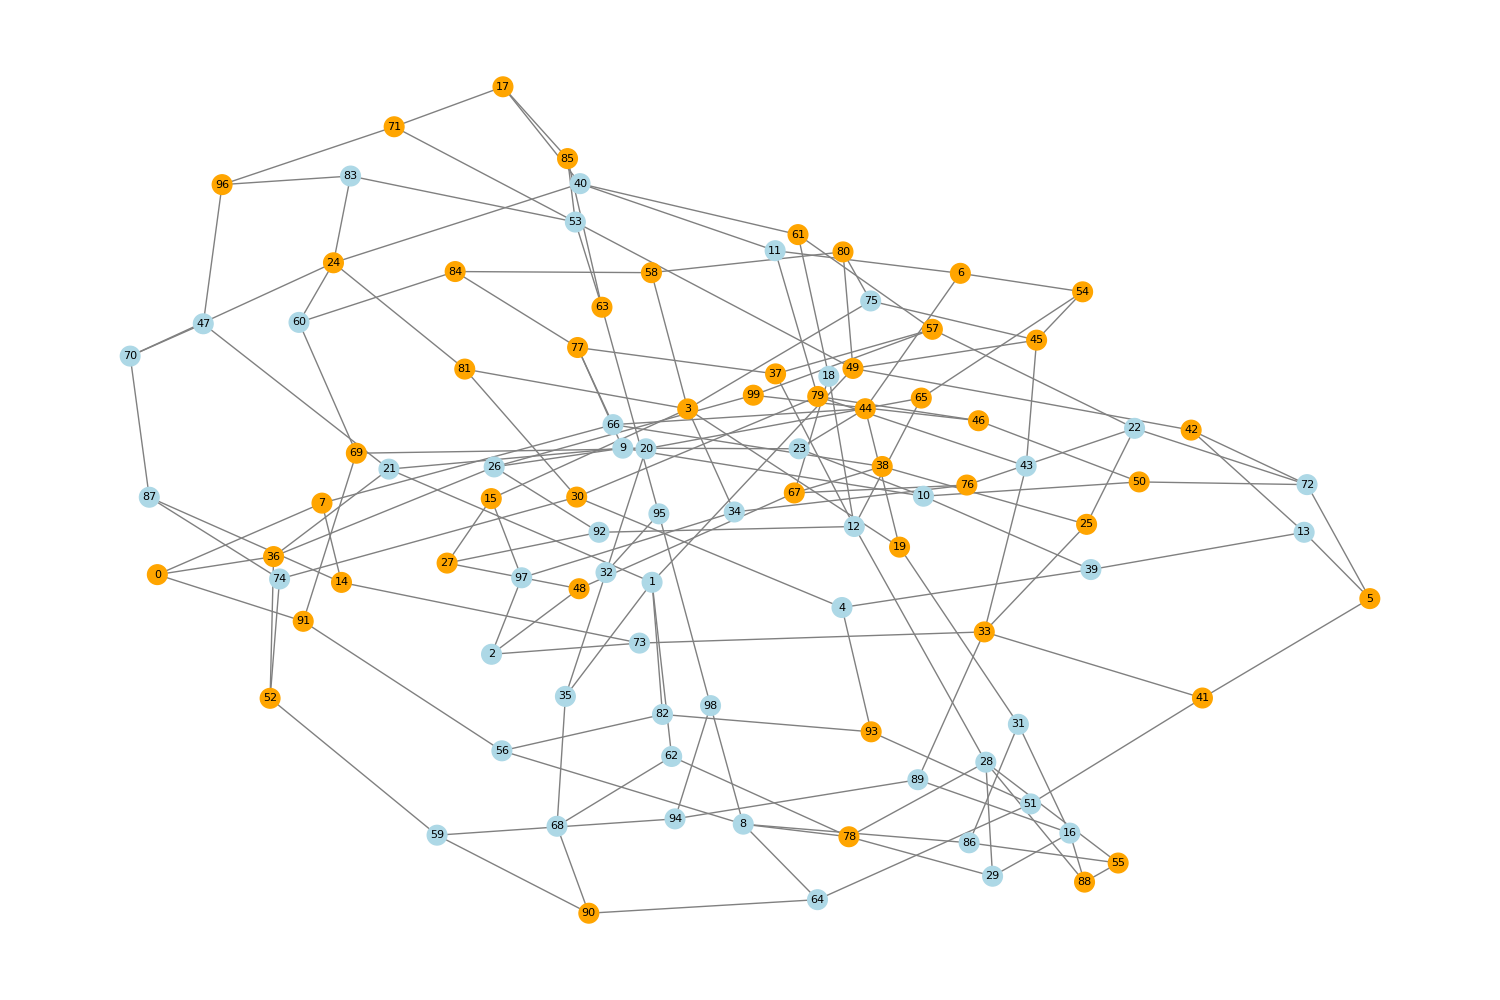
\includegraphics[width=1\textwidth, clip, trim=10 10 10 10]{images/drawNetwork/normal_network.png}} 
	\end{figure}	
	For the same simulation, here is the overlay network:
	\begin{figure}[H]
		\centering
		\fbox{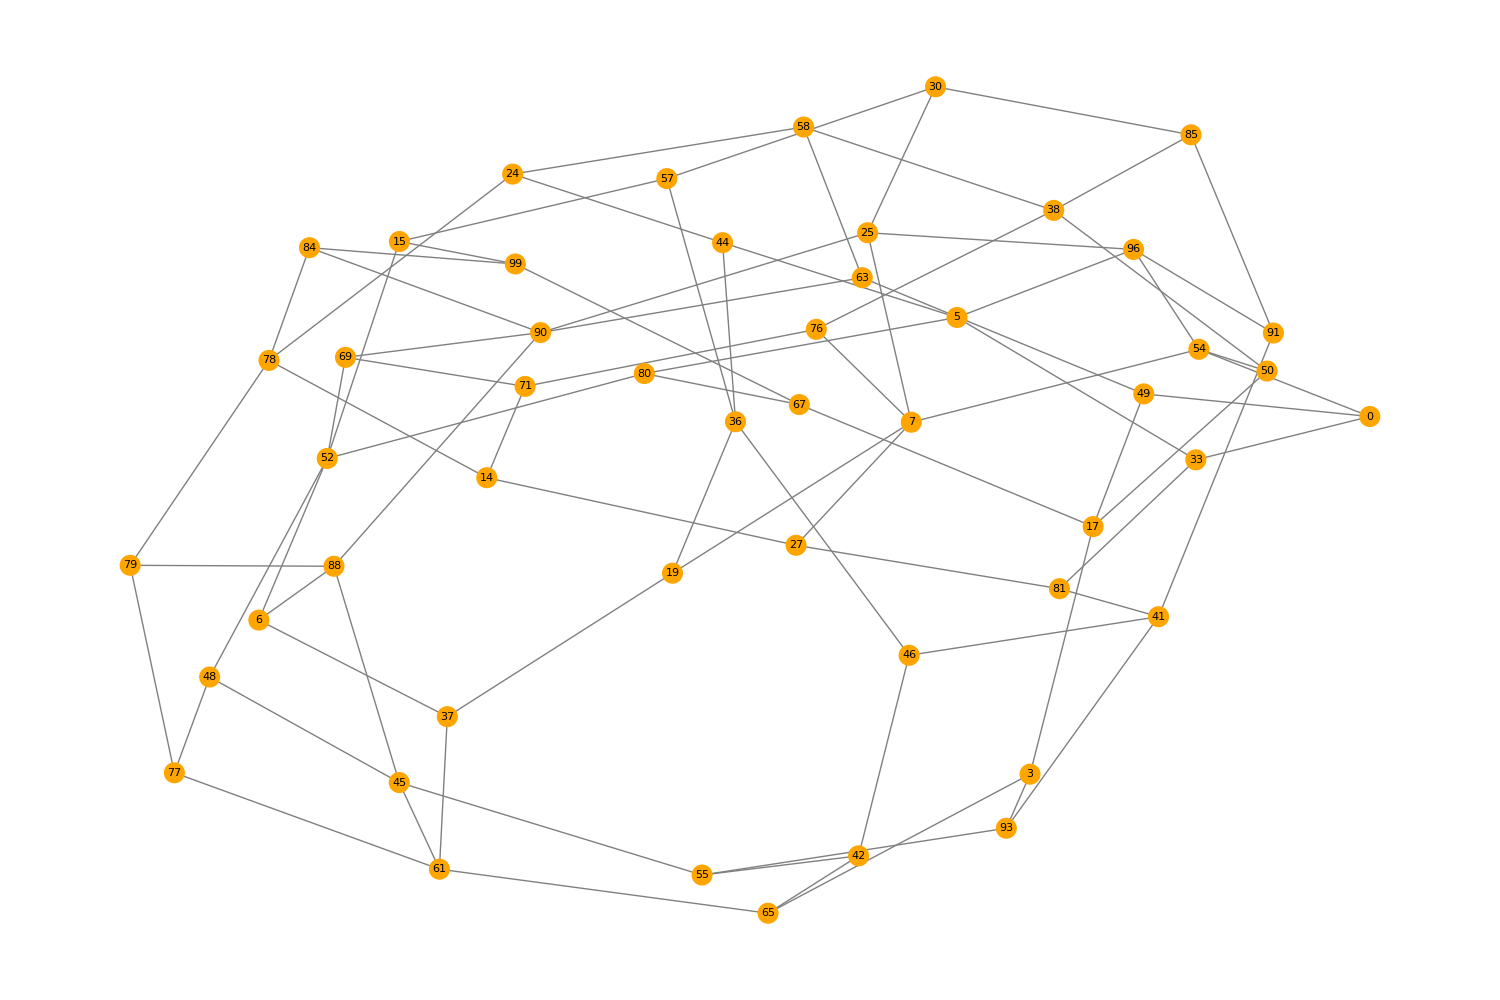
\includegraphics[width=0.5\textwidth, clip, trim=10 10 10 10]{images/drawNetwork/overlay_network.png}} 
	\end{figure}
\end{solution}


\begin{solution}{Theoretical Question Asked}
	In presence of an eclipse attack, increasing the timeout time, affects the block propagation, by allowing the honest nodes, to receive a larger number of other honest blocks. This has many consequences:
	\begin{itemize}
		\item Firstly, if that honest node is doing mining, there are chances that it will get forked out, and the peer will have to stop it's mining, and start again on the new leaf node (because in the meantime, that node has received a block due to a larger timeout).
		\item Because of the above chaos, some of the honest nodes cannot contribute to the longest chain, and this is taken as an advantage to the malicious nodes (primarily ringmaster), which has access to faster information, through the overlay network.
		\item The benefit to the malicious nodes, is clear from the ratios calculated above, which increases as the timeout values increase.
	\end{itemize}

	We also present the trend across these timeout values, for various malicious percentages:
	\begin{figure}[H]
		\centering
		\fbox{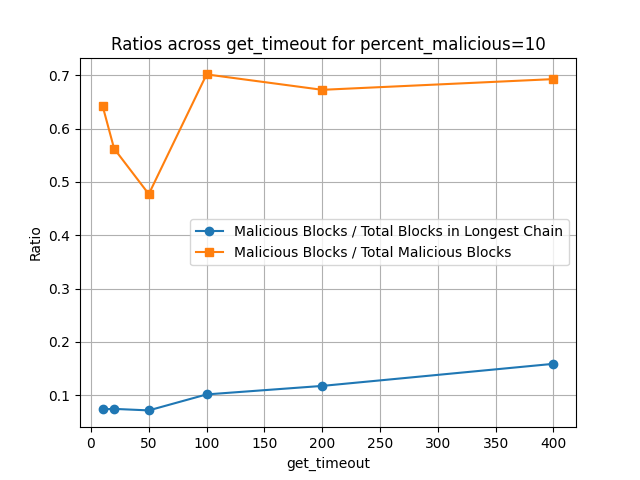
\includegraphics[width=0.5\textwidth, clip, trim=10 10 10 10]{images/get_timeout_vs_ratios_percent_malicious_10.png}} 
		\caption{For malicious percentage=10\%}
	\end{figure}
	\begin{figure}[H]
		\centering
		\fbox{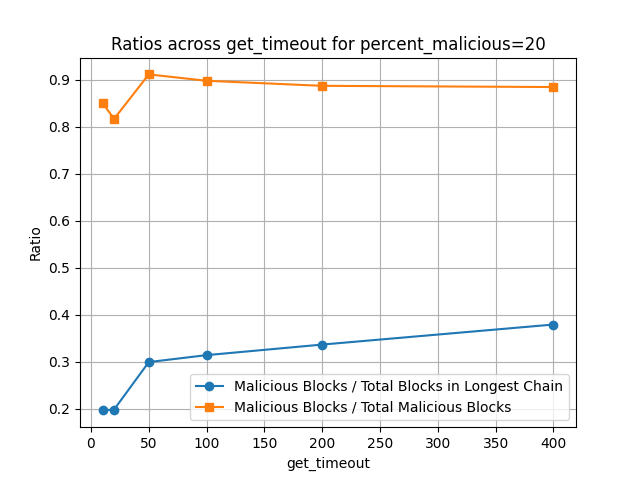
\includegraphics[width=0.5\textwidth, clip, trim=10 10 10 10]{images/get_timeout_vs_ratios_percent_malicious_20.png}} 
		\caption{For malicious percentage=20\%}
	\end{figure}
	\begin{figure}[H]
		\centering
		\fbox{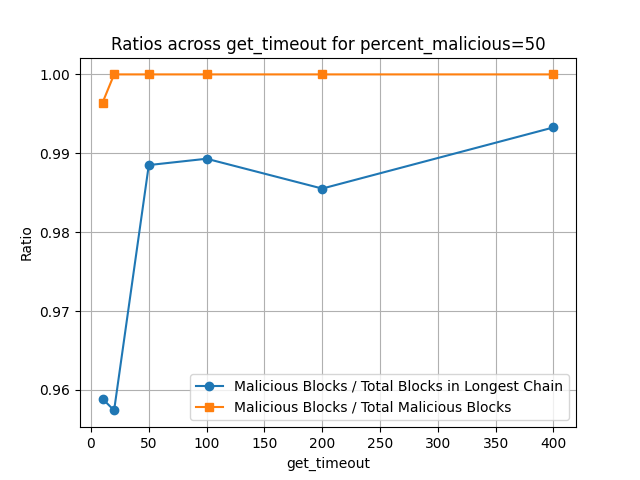
\includegraphics[width=0.5\textwidth, clip, trim=10 10 10 10]{images/get_timeout_vs_ratios_percent_malicious_50.png}} 
		\caption{For malicious percentage=50\%}
	\end{figure}
	\begin{figure}[H]
		\centering
		\fbox{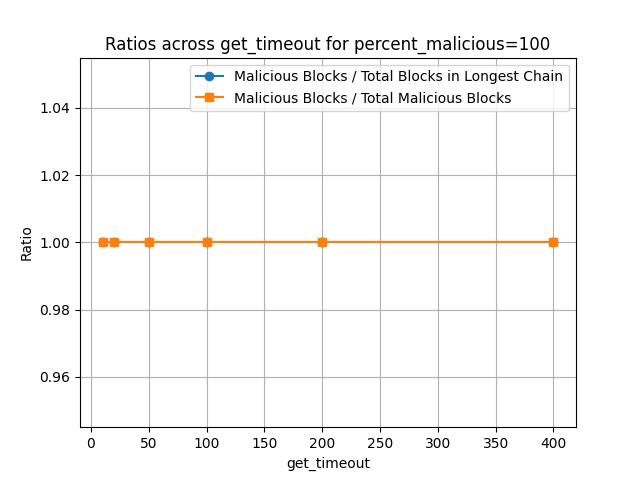
\includegraphics[width=0.5\textwidth, clip, trim=10 10 10 10]{images/get_timeout_vs_ratios_percent_malicious_100.png}} 
		\caption{For malicious percentage=100\%}
	\end{figure}
	An important counter measure has been suggested below.
\end{solution}
\begin{solution}{Countermeasure to Mitigate Attack}
\begin{itemize}
	\item Each honest peer maintains a trust score for its neighbours, which reflects the frequency of successful responses to the peer's requests within the timeout period.
	\begin{mdframed}[linecolor=black, linewidth=2pt, roundcorner=10pt, backgroundcolor=yellow!10!white, skipabove=12pt, skipbelow=12pt]
		\begin{verbatim}
trustScore: Map from neigbour_id to scor
pastAttempts: Map from neigbour_id to pair<successful, total> attempts 
		\end{verbatim}
		\end{mdframed}
	\item A neighbour's trust score decreases when it fails to respond and increases when it\\ successfully responds to a request.
	\begin{mdframed}[linecolor=black, linewidth=2pt, roundcorner=10pt, backgroundcolor=yellow!10!white, skipabove=12pt, skipbelow=12pt]
		\begin{verbatim}
handleFailedRequest(sender_id) {
	trustScore[sender_id] -= 10;
	trustScore[sender_id] = max(0.0, trustScore[sender_id]);

	pastAttempts[sender_id].second += 1;
	pastAttempts[sender_id].first -= 1;
	pastAttempts[sender_id].first = max(0, pastAttempts[sender_id].first);
}

handleSuccesfulRequest(sender_id) {
	trustScore[sender_id] += 1;
	trustScore[sender_id] = min(maxTrustScore, trustScore[sender_id]);

	pastAttempts[sender_id].second += 1;
	pastAttempts[sender_id].first += 1;
}
		\end{verbatim}
		\end{mdframed}
	\item The trust score serves as a relative index among the peer's neighbours.
	\item Neighbours with lower trust scores are deprioritized, causing the peer to delay sending requests to them, giving preference to neighbours with higher trust scores who are more likely to provide the required block hash.
	\begin{mdframed}[linecolor=black, linewidth=2pt, roundcorner=10pt, backgroundcolor=yellow!10!white, skipabove=12pt, skipbelow=12pt]
		\begin{verbatim}
getTrustDelay(sender_id) {
	successRatio = 
		pastAttempts[sender_id].first / pastAttempts[sender_id].second;

	max_delay = maxTrustDelay();
	delay = 
		max_delay * (1 - successRatio * trustScore[sender_id] / maxTrustScore);
	
	return delay;
}
		\end{verbatim}
		\end{mdframed}
	
	\item Neighbours with trustScore less than a threshold are not considered by the peer for the purpose of requesting blocks on receiving hashes and for sending the blocks when a request is received for a fixed number of times. After that the trustScore of the blacklisted node is reset and the node can again communicate with our peer.
	\begin{mdframed}[linecolor=black, linewidth=2pt, roundcorner=10pt, backgroundcolor=yellow!10!white, skipabove=12pt, skipbelow=12pt]
		\begin{verbatim}
RECEIVE_HASH:
if(trustScore[sender_id] > 20) {
		delayedRequestTime = getCurrentTime() + getTrustDelay(sender_id);
		hash_to_timeout[hash] = GetRequestTimeout + delayedRequestTime;
		sendDelayedGetRequest(hash, sender_id, delayedRequestTime); 

} else {
	banCount[sender_id] += 1;
	if(banCount[sender_id] > 5) {
			resetScore(sender_id);
			banCount[sender_id] = 0;
	}
}

SEND_BLOCK:
if(trustScore[targetPeerID] > 20) {
		delayedSendTime = getCurrentTime() + getTrustDelay(targetPeerID);
		scheduleEvent(delayedSendTime, BLOCK_SEND, id, targetPeerID, block);

} else {
	banCount[targetPeerID] += 1;
	if(banCount[targetPeerID] > 5) {
			resetScore(targetPeerID);
			banCount[targetPeerID] = 0;
	}
}

\end{verbatim}
\end{mdframed}

The delay after receiving a hash helps in overcomming the eclipse attack by sending immediate GetBlock requests only to trusted (honest) neighbours. It also helps to some extent towards the Selfish mining attack by not accepting immediately the blocks mined by ringmaster and continue mining on the current leaf node.

\begin{mdframed}[linecolor=black, linewidth=2pt, roundcorner=10pt, backgroundcolor=yellow!10!white, skipabove=12pt, skipbelow=12pt]
	\begin{verbatim}

resetScore(neighbour_id) {
		trustScore[neighbour_id] = maxTrustScore;
		pastAttempts[neighbour_id] = pair<int, int>(1, 1);
}
	\end{verbatim}
	\end{mdframed}
\end{itemize}

\end{solution}

\begin{solution}{Analysis of Countermeasure Strategy}
Consider the case:
\begin{itemize}
	\vspace{-7pt}
	\item Total Peers: 100
	\vspace{-7pt}
	\item Malicious Peers: 30
	\vspace{-7pt}
	\item Block Interarrival Time: 100
	\vspace{-7pt}
	\item Transaction Interarrival Time: 10
	\vspace{-7pt}
	\item GetRequest Timeout: 50 
	\vspace{-7pt}
	\item Time of Execution: 10000
\end{itemize}



\textbf{Countermeasure Disabled}
\begin{figure}[H]
\centering
\fbox{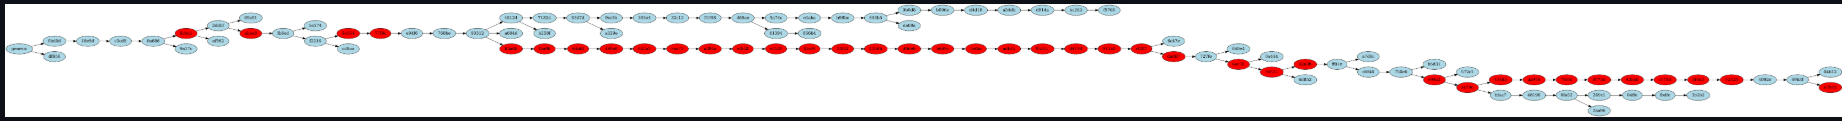
\includegraphics[width=1\textwidth, clip, trim=10 10 10 10]{images/i_woc_30_50.png}} 

\end{figure}
\vspace{-15pt}
\texttt{Malicious Chain: 40 | Total Blocks Chain: 56 | Total Malicious: 40\\
Malicious Blocks in Chain / Total Blocks in Longest Chain: 0.714286\\
Malicious Blocks in Chain / Total Malicious Blocks: 1}\\
% \vspace{15pt}
\textbf{Countermeasure Enabled}
\vspace{0pt}
\begin{figure}[H]
\centering
\fbox{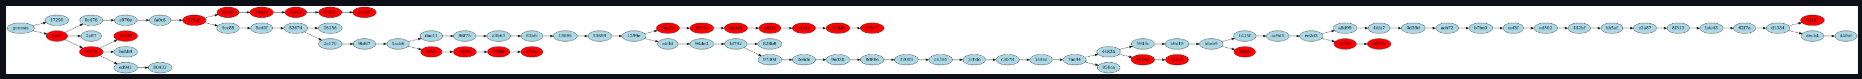
\includegraphics[width=1\textwidth, clip, trim=10 10 10 10]{images/i_wc_30_50.png}} 

\end{figure}
\vspace{-15pt}
\texttt{Malicious Chain: 2 | Total Blocks Chain: 54 | Total Malicious: 26\\
Malicious Blocks in Chain / Total Blocks in Longest Chain: 0.037037\\
Malicious Blocks in Chain / Total Malicious Blocks: 0.0769231}\\

\newpage
Above are the blockchain of the ringmaster in the two cases. Let's see how the countermeasure was able to perform against the attack:\\

- Consider a part of the network as shown: 
\begin{figure}[H]
\centering
\fbox{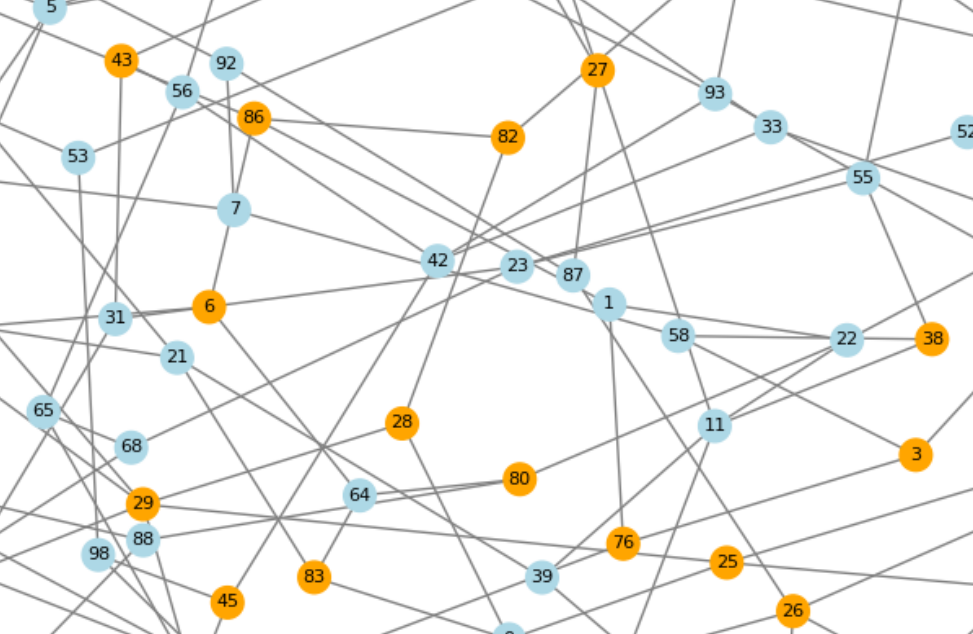
\includegraphics[width=0.6\textwidth, clip, trim=10 10 10 10]{images/i_wc_30_50_net.png}} 
\end{figure}
\begin{itemize}
	\item For Peer 58 the trustScore of its neighbours at end: \\
	3: Score = 50.000000 | H = 9 17\\
	7: Score = 100.000000 | H = 59 59\\
	38: Score = 72.000000 | H = 11 19\\
	This indicates that the peer was able to identify the malicious neighbours and therefore requested most of the blocks from the only honest neigbour (7). \textit{Here H 9 17 indicates that out of 17 times the peer requested block 9 times the neighbour responded \textbf{since reset}.}
	
	\item For Peer 87 the trustScore's are:\\
	26: Score = 91.000000 | H = 13 17\\
	27: Score = 48.000000 | H = 6 16\\
	92: Score = 100.000000 | H = 61 61

	\item For Peer 1 the trustScore's are:\\
	22: Score = 100.000000 | H = 60 60\\
	76: Score = 80.000000 | H = 9 14\\
	86: Score = 91.000000 | H = 12 16

\end{itemize}

This clearly shows that the peers are able to bypass the eclipse attack due to proper identification of the malicious neighbours because if it was not the case then most of requests would be to the malicious neighbours due to low latencies and faster tranmission in overlay network.\\

- Peer 57
\begin{figure}[H]
	\centering
	\fbox{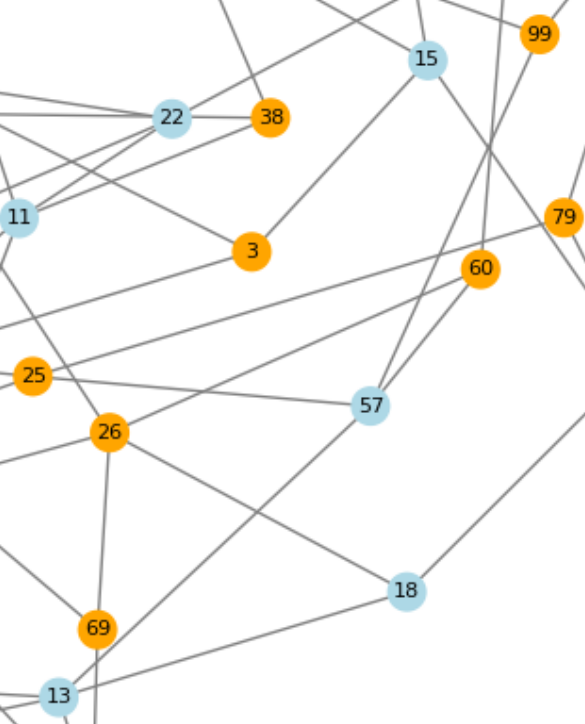
\includegraphics[width=0.3\textwidth, clip, trim=10 10 10 10]{images/peer57.png}} 
\end{figure}
Peer 57 has 3 malicious neighbours [99, 60, 25] and just one honest neighbour [13]. Even after that the chain of the peer is completly synced with the ringmaster's chain.\\\\
13: Score = 100.000000 | H = 60 60\\
25: Score = 81.000000 | H = 11 17\\
60: Score = 63.000000 | H = 2 8\\
99: Score = 77.000000 | H = 6 11

\begin{figure}[H]
	\centering
	\fbox{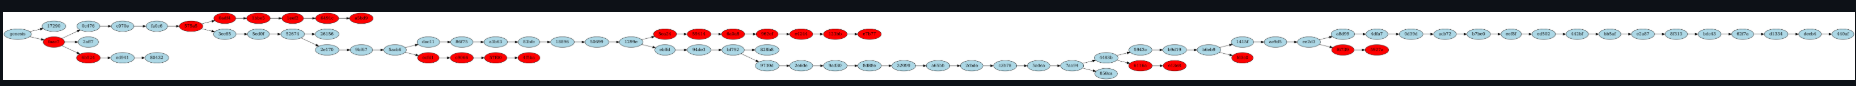
\includegraphics[width=1\textwidth, clip, trim=10 10 10 10]{images/peer57_chain.png}} 
\end{figure}

\textbf{More Runs:}
\begin{itemize}
	\vspace{-7pt}
	\item Total Peers: 100
	\vspace{-7pt}
	\item Malicious Peers: 40
	\vspace{-7pt}
	\item Block Interarrival Time: 100
	\vspace{-7pt}
	\item Transaction Interarrival Time: 10
	\vspace{-7pt}
	\item GetRequest Timeout: 100 
	\vspace{-7pt}
	\item Time of Execution: 100000
\end{itemize}

\textbf{Countermeasure Disabled}
\begin{figure}[H]
\centering
\fbox{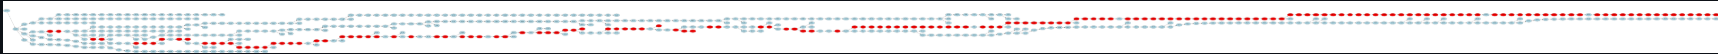
\includegraphics[width=1\textwidth, clip, trim=10 10 10 10]{images/40_100000_woc.png}} 

\end{figure}
% \vspace{15pt}
\textbf{Countermeasure Enabled}
\vspace{0pt}
\begin{figure}[H]
\centering
\fbox{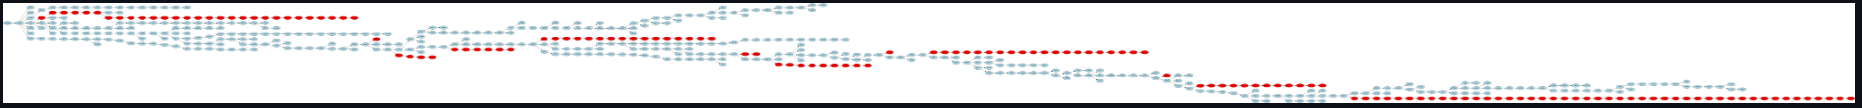
\includegraphics[width=1\textwidth, clip, trim=10 10 10 10]{images/40_100000_wc}} 

\end{figure}

\textbf{More Runs:}
\begin{itemize}
	\vspace{-7pt}
	\item Total Peers: 100
	\vspace{-7pt}
	\item Malicious Peers: 20
	\vspace{-7pt}
	\item Block Interarrival Time: 100
	\vspace{-7pt}
	\item Transaction Interarrival Time: 10
	\vspace{-7pt}
	\item GetRequest Timeout: 40 
	\vspace{-7pt}
	\item Time of Execution: 10000
\end{itemize}

\textbf{Countermeasure Disabled}
\begin{figure}[H]
\centering
\fbox{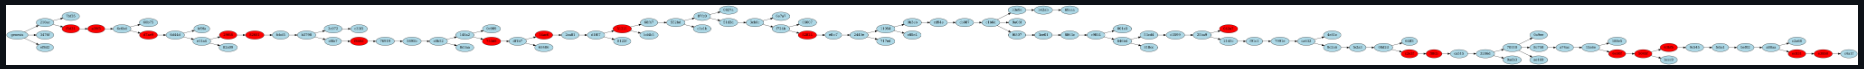
\includegraphics[width=1\textwidth, clip, trim=10 10 10 10]{images/100_20_10_100_40_wo.png}} 

\end{figure}
\vspace{-15pt} 
\texttt{Malicious Chain: 17 |
Total Blocks Chain: 70 |
Total Malicious: 18\\
Malicious Blocks in Chain / Total Blocks in Longest Chain: 0.242857\\
Malicious Blocks in Chain / Total Malicious Blocks: 0.944444}\\

% \vspace{15pt}
\textbf{Countermeasure Enabled}
\vspace{0pt}
\begin{figure}[H]
\centering
\fbox{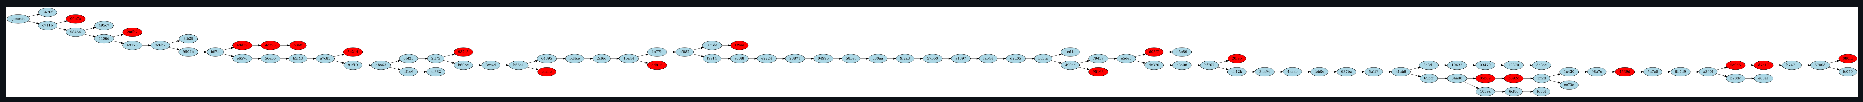
\includegraphics[width=1\textwidth, clip, trim=10 10 10 10]{images/100_20_10_100_40_w.png}} 

\end{figure}
\vspace{-15pt}
\texttt{Malicious Chain: 6 |
Total Blocks Chain: 66 |
Total Malicious: 19 \\
Malicious Blocks in Chain / Total Blocks in Longest Chain: 0.0909091\\
Malicious Blocks in Chain / Total Malicious Blocks: 0.315789}\\

\textbf{More Runs:}
\begin{itemize}
	\vspace{-7pt}
	\item Total Peers: 50
	\vspace{-7pt}
	\item Malicious Peers: 40
	\vspace{-7pt}
	\item Block Interarrival Time: 300
	\vspace{-7pt}
	\item Transaction Interarrival Time: 10
	\vspace{-7pt}
	\item GetRequest Timeout: 80 
	\vspace{-7pt}
	\item Time of Execution: 40000
\end{itemize}



\textbf{Countermeasure Disabled}
\begin{figure}[H]
\centering
\fbox{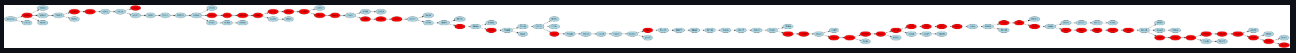
\includegraphics[width=1\textwidth, clip, trim=10 10 10 10]{images/50_40_10_300_80_40000_wo.png}} 

\end{figure}
\vspace{-15pt}
\texttt{Malicious Chain: 47 |
Total Blocks Chain: 82 |
Total Malicious: 48\\
Malicious Blocks in Chain / Total Blocks in Longest Chain: 0.573171\\
Malicious Blocks in Chain / Total Malicious Blocks: 0.979167}\\

\textbf{Countermeasure Enabled}
\vspace{0pt}
\begin{figure}[H]
\centering
\fbox{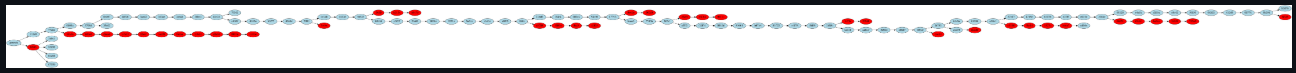
\includegraphics[width=1\textwidth, clip, trim=10 10 10 10]{images/50_40_10_300_80_40000_w.png}} 

\end{figure}
\vspace{-15pt}
\texttt{Malicious Chain: 1 |
Total Blocks Chain: 70 |
Total Malicious: 39\\
Malicious Blocks in Chain / Total Blocks in Longest Chain: 0.0142857\\
Malicious Blocks in Chain / Total Malicious Blocks: 0.025641}\\

\textbf{More Runs:}
\begin{itemize}
	\vspace{-7pt}
	\item Total Peers: 100
	\vspace{-7pt}
	\item Malicious Peers: 40
	\vspace{-7pt}
	\item Block Interarrival Time: 100
	\vspace{-7pt}
	\item Transaction Interarrival Time: 10
	\vspace{-7pt}
	\item GetRequest Timeout: 60 
	\vspace{-7pt}
	\item Time of Execution: 30000
\end{itemize}



\textbf{Countermeasure Disabled}
\begin{figure}[H]
\centering
\fbox{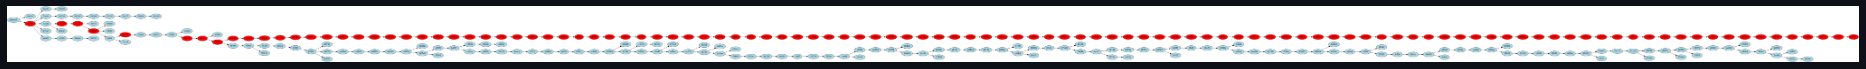
\includegraphics[width=1\textwidth, clip, trim=10 10 10 10]{images/100_40_10_100_40_wo.png}} 

\end{figure}
\vspace{-15pt}
\texttt{Malicious Chain: 112 |
Total Blocks Chain: 117 |
Total Malicious: 112\\
Malicious Blocks in Chain / Total Blocks in Longest Chain: 0.957265\\
Malicious Blocks in Chain / Total Malicious Blocks: 1}\\

\textbf{Countermeasure Enabled}
\vspace{0pt}
\begin{figure}[H]
\centering
\fbox{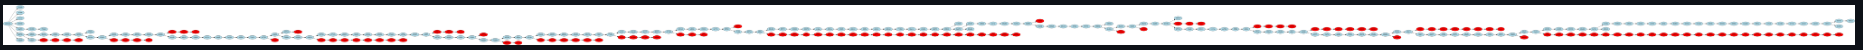
\includegraphics[width=1\textwidth, clip, trim=10 10 10 10]{images/100_40_10_100_60_w.png}} 

\end{figure}
\vspace{-15pt}
\texttt{Malicious Chain: 0 |
Total Blocks Chain: 159 |
Total Malicious: 115\\
Malicious Blocks in Chain / Total Blocks in Longest Chain: 0\\
Malicious Blocks in Chain / Total Malicious Blocks: 0}\\

\end{solution}


\begin{solution}{Analysis over various Blockchain Trees}
	Based on the flags provided (\texttt{--blockchain} or \texttt{--dump-all}), our code generates blockchain trees of the nodes of the network. Here we will analyze the blockchain trees of ringMaster:

	% \begin{figure}[H]
	% 	\centering
	% 	\fbox{
\includegraphics[width=1\textwidth]{images/ringmaster_100_100_10_100_100_10000_no_eclipse.png}} 
	% \end{figure}
	\textbf{Eclipse + Selfish Mining}\\
	\begin{itemize}
		\item \begin{itemize}
			\vspace{-7pt}
			\item Total Peers: 100
			\vspace{-7pt}
			\item Malicious Peers: 5
			\vspace{-7pt}
			\item Block Interarrival Time: 100
			\vspace{-7pt}
			\item Transaction Interarrival Time: 10
			\vspace{-7pt}
			\item GetRequest Timeout: 50 
			\vspace{-7pt}
			\item Time of Execution: 17500
		\end{itemize}
		 \begin{figure}[H]
				\centering
				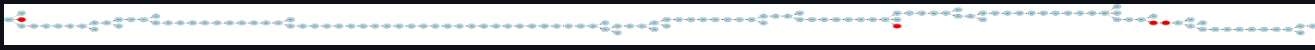
\includegraphics[width=\textwidth]{images/i_100_5_10_100_50_SE.png} 
			\end{figure}
			\item \begin{itemize}
				\vspace{-7pt}
				\item Total Peers: 100
				\vspace{-7pt}
				\item Malicious Peers: 10
				\vspace{-7pt}
				\item Block Interarrival Time: 100
				\vspace{-7pt}
				\item Transaction Interarrival Time: 10
				\vspace{-7pt}
				\item GetRequest Timeout: 50 
				\vspace{-7pt}
				\item Time of Execution: 17500
			\end{itemize}
			 \begin{figure}[H]
					\centering
					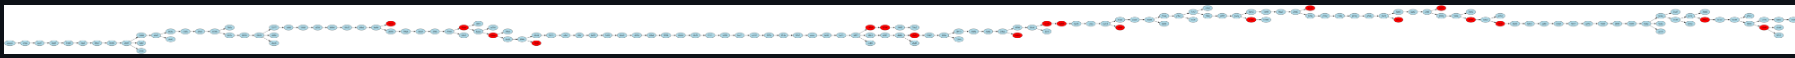
\includegraphics[width=\textwidth]{images/i_100_10_10_100_50_SE.png} 
				\end{figure}
		
				\item \begin{itemize}
					\vspace{-7pt}
					\item Total Peers: 100
					\vspace{-7pt}
					\item Malicious Peers: 15
					\vspace{-7pt}
					\item Block Interarrival Time: 100
					\vspace{-7pt}
					\item Transaction Interarrival Time: 10
					\vspace{-7pt}
					\item GetRequest Timeout: 50 
					\vspace{-7pt}
					\item Time of Execution: 17500
				\end{itemize}
				 \begin{figure}[H]
						\centering
						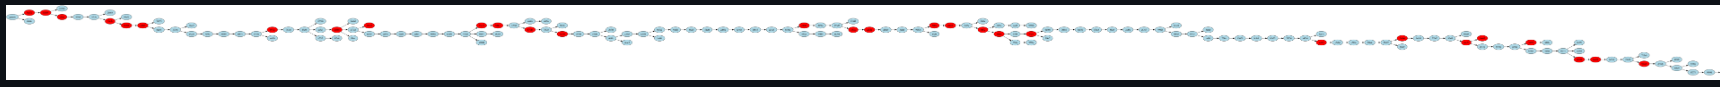
\includegraphics[width=\textwidth]{images/i_100_15_10_100_50_SE.png} 
					\end{figure}
	
	
		\item \begin{itemize}
			\vspace{-7pt}
			\item Total Peers: 100
			\vspace{-7pt}
			\item Malicious Peers: 20
			\vspace{-7pt}
			\item Block Interarrival Time: 100
			\vspace{-7pt}
			\item Transaction Interarrival Time: 10
			\vspace{-7pt}
			\item GetRequest Timeout: 50 
			\vspace{-7pt}
			\item Time of Execution: 17500
		\end{itemize}
		 \begin{figure}[H]
				\centering
				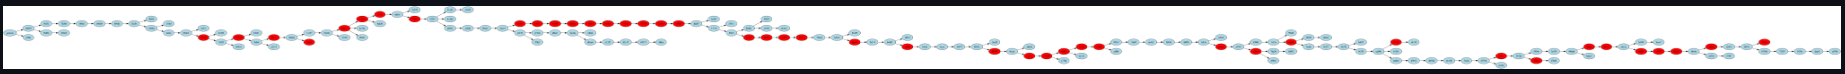
\includegraphics[width=\textwidth]{images/i_100_20_10_100_50_SE.png} 
			\end{figure}
	
	
		\item \begin{itemize}
			\vspace{-7pt}
			\item Total Peers: 100
			\vspace{-7pt}
			\item Malicious Peers: 30
			\vspace{-7pt}
			\item Block Interarrival Time: 100
			\vspace{-7pt}
			\item Transaction Interarrival Time: 10
			\vspace{-7pt}
			\item GetRequest Timeout: 50 
			\vspace{-7pt}
			\item Time of Execution: 17500
		\end{itemize}
	
		 \begin{figure}[H]
				\centering
				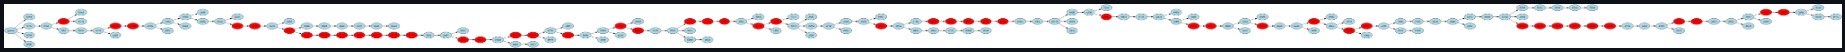
\includegraphics[width=\textwidth]{images/i_100_30_10_100_50_SE.png} 
			\end{figure}
	
			\item \begin{itemize}
				\vspace{-7pt}
				\item Total Peers: 100
				\vspace{-7pt}
				\item Malicious Peers: 40
				\vspace{-7pt}
				\item Block Interarrival Time: 100
				\vspace{-7pt}
				\item Transaction Interarrival Time: 10
				\vspace{-7pt}
				\item GetRequest Timeout: 50 
				\vspace{-7pt}
				\item Time of Execution: 17500
			\end{itemize}
		
			 \begin{figure}[H]
					\centering
					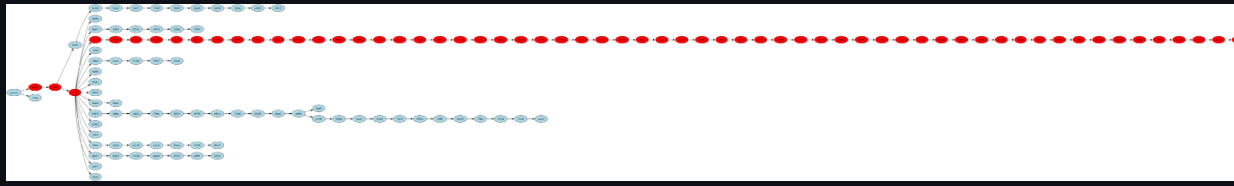
\includegraphics[width=\textwidth]{images/i_100_40_10_100_50_SE.png} 
				\end{figure}
	
	
					\item \begin{itemize}
						\vspace{-7pt}
						\item Total Peers: 100
						\vspace{-7pt}
						\item Malicious Peers: 60
						\vspace{-7pt}
						\item Block Interarrival Time: 100
						\vspace{-7pt}
						\item Transaction Interarrival Time: 10
						\vspace{-7pt}
						\item GetRequest Timeout: 50 
						\vspace{-7pt}
						\item Time of Execution: 17500
					\end{itemize}
				
					 \begin{figure}[H]
							\centering
							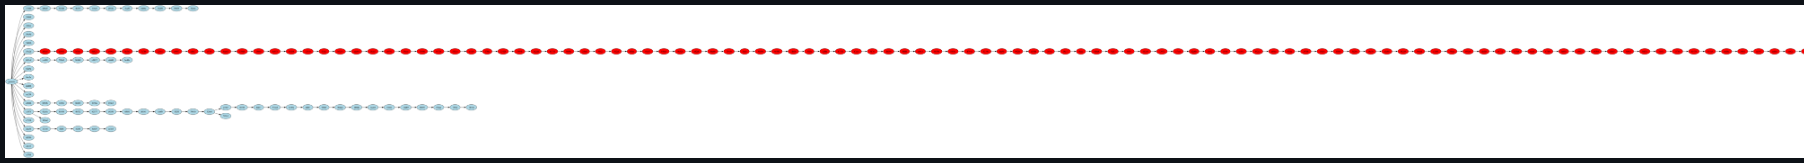
\includegraphics[width=\textwidth]{images/i_100_60_10_100_50_SE.png} 
						\end{figure}
	
		\item \begin{itemize}
			\vspace{-7pt}
			\item Total Peers: 100
			\vspace{-7pt}
			\item Malicious Peers: 40
			\vspace{-7pt}
			\item Block Interarrival Time: 100
			\vspace{-7pt}
			\item Transaction Interarrival Time: 10
			\vspace{-7pt}
			\item GetRequest Timeout: 20 
			\vspace{-7pt}
			\item Time of Execution: 17500
		\end{itemize}
	
			\begin{figure}[H]
				\centering
				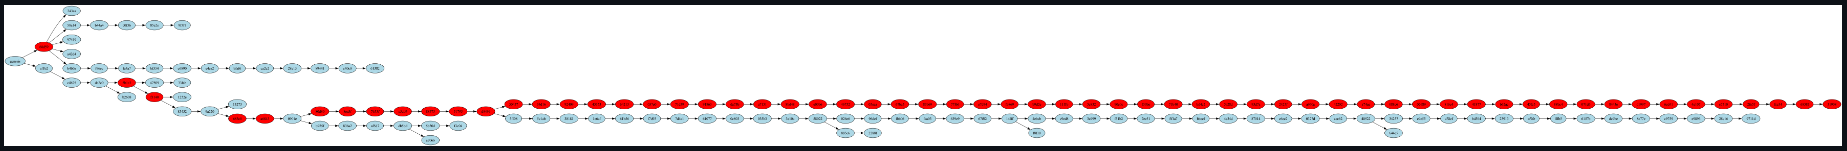
\includegraphics[width=\textwidth]{images/i_100_40_10_100_20_SE.png} 
			\end{figure}
		\item \begin{itemize}
			\vspace{-7pt}
			\item Total Peers: 100
			\vspace{-7pt}
			\item Malicious Peers: 50
			\vspace{-7pt}
			\item Block Interarrival Time: 100
			\vspace{-7pt}
			\item Transaction Interarrival Time: 10
			\vspace{-7pt}
			\item GetRequest Timeout: 100 
			\vspace{-7pt}
			\item Time of Execution: 17500
		\end{itemize}
			\begin{figure}[H]
				\centering
				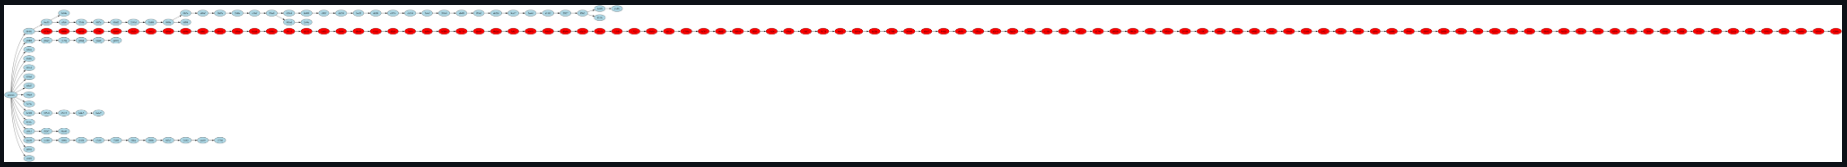
\includegraphics[width=\textwidth]{images/i_100_50_10_100_100_SE.png} 
			\end{figure}
	\end{itemize}	
	
	
	

\end{solution}
\end{document}
